\section{Analisis Sisi Pasokan}
\label{sec:supply-side-analysis}

\subsection{Batasan Sarat Pelabuhan}
\label{subsec:batasan-sarat-pelabuhan}

Salah satu aspek utama yang harus diperhatikan dalam merencakan armada transportasi laut adalah kedalaman pelabuhan. Kebanyakan pelabuhan di Maluku Barat Daya memiliki kedalaman rendah. Kemudian karena faktor pelabuhan pesisir maka kedalaman yang ada harus diberi \emph{margin} untuk mengantisipasi ketika terjadi surut sehingga kedalaman pelabuhan berkurang.

\begin{table}[!htbp]
    \centering
    \caption{Data Kedalaman Pelabuhan}
    \begin{tabular}{|l|l|}
    \hline
        Nama Pelabuhan & \emph{Draft} (m) \\ \hline
        TBBM Saumlaki & 10 \\ \hline
        Pelabuhan Kaiwatu & 7 \\ \hline
        Pelabuhan Moa & 6.6 \\ \hline
        Pelabuhan Lakor & 5 \\ \hline
        Pelabuhan Romang & 4.9 \\ \hline
        Pelabuhan Letti & 5.2 \\ \hline
    \end{tabular}
    \label{tabel-draft-port}
\end{table}

\subsection{Variasi Durasi Gangguan Cuaca}
\label{subsec:variasi-Durasi-gangguan-cuaca}

Elemen kedua dari model yang divariasikan adalah durasi gangguan cuaca. Variabel ini dan interaksinya dengan konsumsi harian akan memberikan indikator jika terjadi \emph{stock out} BBM di suatu titik. Data historis yang dijadikan penentuan distribusi durasi gangguan cuaca adalah data yang penulis dapati dari situs berita mengenai lama gangguan cuaca beberapa tahun terakhir di Kabupaten Maluku Barat Daya.

Fungsi yang digunakan untuk memodelkan durasi gangguan cuaca adalah \emph{IntUniform} dengan nilai minimum 7 hari dan nilai maksimum yang diambil untuk simulasi adalah 46 hari. Digunakan distribusi seragam karena tidak diketahui seberapa besar kemungkinan gangguan cuaca untuk durasinya, Sehingga diambil peluang semua nilai adalah sama. Grafik distribusi kumulatif gangguan cuaca dapat dilihat pada gambar \ref{fig:grafik-kumulatif-durasi-gangguan-cuaca-1st}.

\begin{figure}[htbp!]
    \centering
    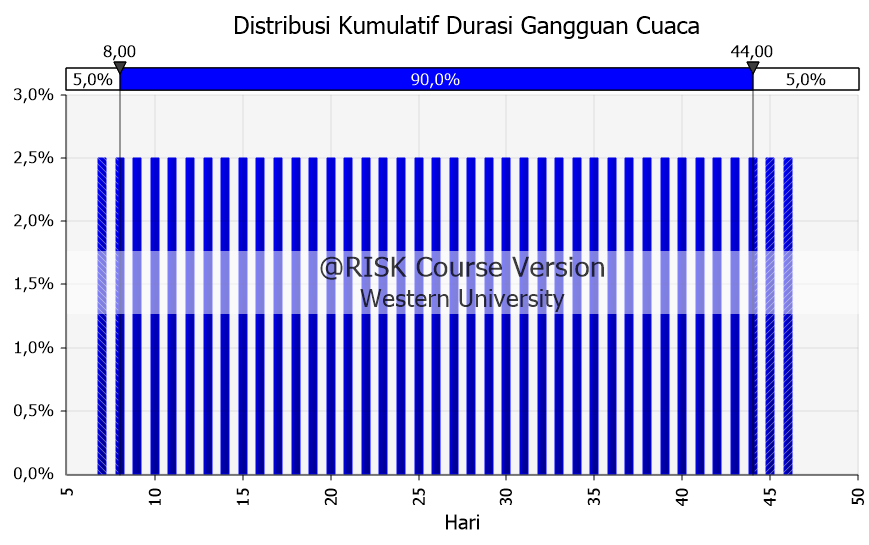
\includegraphics[width=0.8\textwidth]{gambar/graf-kumulatif-cuaca-awal.png}
    \caption{Grafik Distribusi Kumulatif Durasi Gangguan Cuaca}
    \label{fig:grafik-kumulatif-durasi-gangguan-cuaca-1st}
\end{figure}

\subsection{Usulan Rute Pemasokan Baru}
\label{subsec:usulan-rute-baru}

    Sistem pemasokan BBM baru yang diusulkan menggunakan sistem \emph{multiport} dengan cara menyinggahi seluruh titik pemasokan dalam satu perjalanan. Kompromi yang harus dilakukan kapasitas kapal harus besar karena membawa seluruh kebutuhan BBM untuk semua titik. Namun, \emph{trade off} yang muncul adalah berkurangnya jumlah frekuensi pemasokan yang berdampak pada berkurangnya biaya BBM dan biaya pelabuhan yang harus dikeluarkan.

\begin{figure}[htbp!]
    \centering
    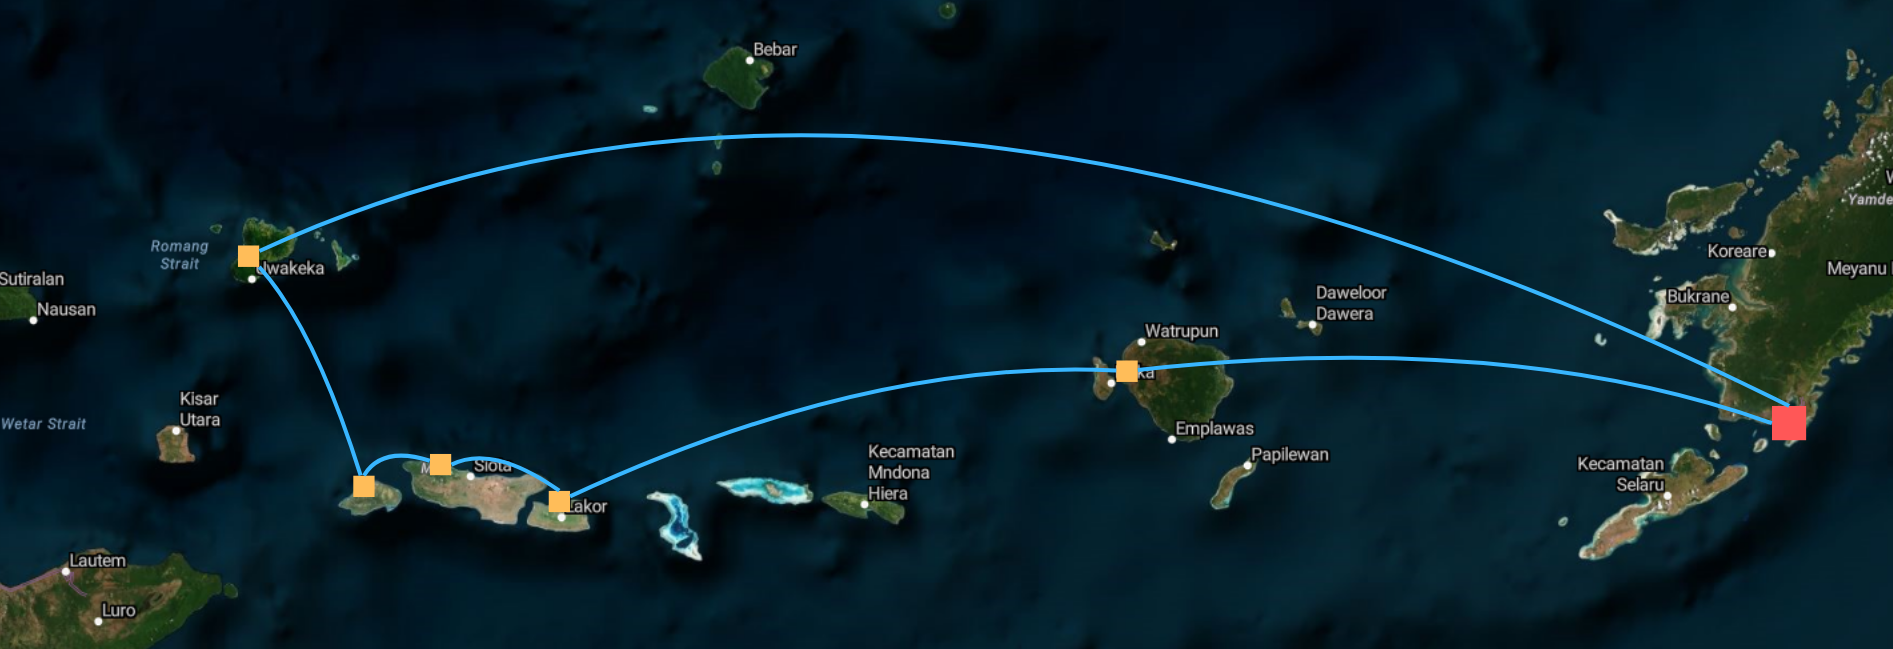
\includegraphics[width=0.8\textwidth]{gambar/rute-baru.png}
    \caption{Gambar Ilustrasi Rute Pemasokan Baru}
    \label{fig:rute-baru}
\end{figure}

    Rute baru yang dirancang dimulai dari TBBM Saumlaki menuju Tepa, Lakor, Tiakur, Letti dan Romang kemudian kembali lagi ke Saumlaki. Rute ini mempunyai jarak totak 522.6 Nm. Namun dibandingkan dengan sistem \emph{direct} dari TBBM Saumlaki akan sangat jauh karena lokasi TBBM Saumlaki yang berada jauh di timur lokasi pemasokan.